\section{Mathematical Model}
\label{sec:mathmod}

To model an infinitely long 3D waveguide \textit{in silico}, the simulation domain must be divided up into regions where specific mathematical relations hold. In this particular system there are three such regions (1) PEC surrounded dielectric, (2) Total Field / Scattered Field (TF/SF) 1-way source, and (3) Mur Absorbing Boundary Condition (Mur ABC). Regions (2)-(3) are essential in making the waveguide appear infinite in length to a propagating wave. A high level diagram of an infinite, PEC bordered rectangular waveguide can be found in Fig. \ref{fig:model}(a) and a $\hat{y}$ sliced model where said relations hold can be found in Fig. \ref{fig:model}(b). These governing relations are then discretized to formulate time-stepping formulas which allow the system to evolve transiently.

\begin{figure}[t!]  
	\centering
	%the command within the [] sets the width of the figure, stability-condition is the jpg name
	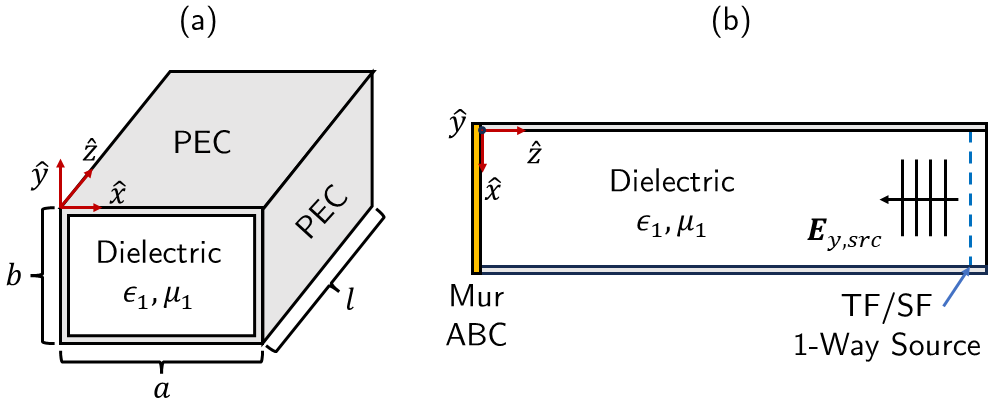
\includegraphics[width=0.9\linewidth]{model} 
	\caption{Diagrams of (a) High-Level PEC Rectangular Waveguide (b) $\hat{y}$-Sliced Model with Labeled Regions}
	\label{fig:model}
\end{figure}

\subsection{Model Formulation}
\label{subsec:model-formulation}

\subsubsection{PEC Surrounded Dielectric}
\label{subsec:dielectric-formulation}

As outlined in Fig. \ref{fig:model}(b) the vast majority of the simulation domain is composed of a PEC enclosed dielectric, the governing equations of which are Amp\`{e}re's and Faraday's Laws respectively. In differential form, these equations take the form 
\begin{align}
    \nabla\times\textbf{H} = \frac{\partial\textbf{D}}{\partial t} + \textbf{J}
    \label{eq:ampere}
\end{align}
and 
\begin{align}
    \nabla\times\textbf{E}=-\frac{\partial\textbf{B}}{\partial t} - \textbf{M}
    \label{eq:faraday}
\end{align}
where \textbf{E} is the electric field, \textbf{D} is the electric flux density, \textbf{H} is the electric field, \textbf{B} is the magnetic flux density, \textbf{J} is the free electric current density, and \textbf{M} is the fictitious free magnetic current density.

For simplicity, this analysis focuses on diagonally-isotropic, time-invariant, and non-dispersive dielectrics within the waveguide. Under these stipulations, each set of fields and flux densities, (\textbf{E}, \textbf{D}), (\textbf{H}, \textbf{B}), can be related using the following constitutive relations
\begin{align}
	\textbf{D}=\epsilon\textbf{E}, \textbf{B}=\mu\textbf{H}
	\label{eq:cor}
\end{align}
with $\epsilon$ and $\mu$ as the permittivity and permeability of the dielectric respectively.

In this analysis, no fictitious magnetic conductors will be considered as they are not pertinent, thus $\textbf{M} = 0$. The free electric current density is treated as a linear superposition of Ohmic conduction $\textbf{J}_{Ohm}=\sigma\textbf{E}$ and and a source term $\textbf{J}_{src}$
\begin{align}
	\textbf{J} = \sigma\textbf{E} + \textbf{J}_{src}
	\label{eq:current}
\end{align}
where $\sigma$ is the diagonally-isotropic, time-invariant dielectric conductivity. In the described system, the inclusion of both a source current density and ohmic current density is not necessary as the wave is assumed to already be propagating in the waveguide from the TF/SF source, and Ohmic losses result in evanescent wave propagation along the waveguide's length. Despite this, these current density terms will be included in the governing set of equations for completeness. The full set of governing equations for waves propogating within the dielectric are as follows
\begin{align}
    \nabla\times\textbf{H} = \epsilon\frac{\partial\textbf{E}}{\partial t} + \sigma\textbf{E} + \textbf{J}_{src}
    \label{eq:ampere-final}
\end{align}
\begin{align}
    \nabla\times\textbf{E}=-\mu\frac{\partial\textbf{H}}{\partial t}.
    \label{eq:faraday-final}
\end{align}

Each of these 3D vector equations can be broken down into $\hat{x}$, $\hat{y}$, and $\hat{z}$ component equations; the $\hat{y}$ components of \textbf{E} and \textbf{H} in Eqs. (\ref{eq:ampere-final})-(\ref{eq:faraday-final}) are
\begin{align}
	\frac{\partial H_x}{\partial z} - \frac{\partial H_z}{\partial x} = \epsilon\frac{\partial E_y}{\partial t} + \sigma E_y + J_{y,src}
	\label{ampere-full-ey}
\end{align}
and
\begin{align}
	\frac{\partial E_x}{\partial z} - \frac{\partial E_z}{\partial x} =-\mu\frac{\partial H_y}{\partial t}
	\label{faraday-full-hy}
\end{align}
respectively.

These scalar equations are valid for all locations within the dielectric region excluding those inside of the PEC at which there is a Dirichlet boundary condition
\begin{align}
	E_x=E_y=0.
	\label{eq:dirichlet}
\end{align}
This Dirichlet boundary condition originates from the conservation of tangential electric fields at medium boundaries 
\begin{align}
	\hat{n}\times\textbf{E}_1=\hat{n}\times\textbf{E}_2.
	\label{eq:electricbc}
\end{align}
By nature of their infinite conductivity, electric fields cannot exist within in the PEC walls thus Eq. (\ref{eq:electricbc}) gives rise to Eq. (\ref{eq:dirichlet}).

\subsubsection{TF/SF 1-way Source}
\label{subsubsec:ftsf-mod}
One of the most popular formulations for injecting source fields into a simulation domain is via a TF/SF 1-way source \cite{taftlovefdtd}. The total-field, scattered-field formulation is built on the linearity of Maxwell's equations. Fields within the total-field region are a superposition of source fields and reflected fields where as fields in the scattered field only consist of those reflected off of materials within the simulation.

As shown in Fig. \ref{fig:model}, The TF/SF source is introduced in a plane with a normal vector $\hat{n}=-\hat{z}$. As outlined in \cite{taftlovefdtd}, fields may be introduced on such planes by fully specifying $E_x, E_y, H_x$ and $H_y$. For this analysis, the waveguide source fields will be restricted to $E_y, H_x$ and $H_z$ as in \cite{fieldsandwavescomm}. Thus for source fields originating on a $\hat{z}$ plane, only the former two fields need to be specified. 

To respect the Dirichlet boundary condition on PEC walls as defined in  Eqs. (\ref{eq:dirichlet}-\ref{eq:electricbc}), the spatial distribution of the steady state frequency solution must be satisfied as to ensure all numerical results are physical. These time independent solutions are as follows
\begin{align}
	E_y=E_0\sin{\frac{\pi x}{a}}
	\label{eq:eyfreq}
\end{align}
and
\begin{align}
	H_x = -\left(\eta\left[1-\left(\frac{\omega_c}{\omega}\right)^2\right]^{-1/2}\right)^{-1}\left(E_0\sin{\frac{\pi x}{a}}\right)
	\label{eq:hxfreq}
\end{align}
where $E_0$ is the initial complex valued waveguide intensity, $a$ is the width of the waveguide as in \ref{fig:model}, $\eta$ is the intrinsic impedance of the waveguide dielectric, $\omega_c$ is the cutoff angular frequency of the waveguide, and $\omega$ is the angular frequency of the source field \cite{fieldsandwavescomm}.

Converting Eqs. (\ref{eq:eyfreq}-\ref{eq:hxfreq}) to the time-domain, the 1-way TF/SF source formulation becomes
\begin{align}
	E_y=E_{y,src}(t)\sin{\frac{\pi x}{a}} + E_{scat}
	\label{eq:tfsf-ey}
\end{align}
and
\begin{multline}
	H_x = -E_{y,src}(t)\left(\eta\left[1-\left(\frac{\omega_c}{\omega}\right)^2\right]^{-1/2}\right)^{-1}\left(\sin{\frac{\pi x}{a}}\right) \\ + H_{scat}
	\label{eq:tfsf-hx}
\end{multline}
in the total field region with $E_{scat}$ as the scattered electric field, $H_{scat}$ as the scattered magnetic field, and $E_{y,src}$ as a time-varying $E_y$ source field. The time-varying source field is specific to the desired simulation outcomes. To obtain a response at a nearly monochromatic frequency, a tapered sine wave may be used 
\begin{align}
	E_{y,src} = E_0\left[1 - \exp{\frac{(t - t_d)}{\tau}}\right]\sin{\omega_0 t}
\end{align}
where $t_d$ is a delay time and $\tau$ is the temporal width of the ramping period. The tapered sine source gradually ramps-up to full field intensity reducing numerical artifacts from sudden jumps \cite{rothlecnotes}.

To obtain a wide-band simulation response, a modulated Gaussian pulse is ideal as it allows for the specification of frequency content via the temporal ramping period witdh $\tau$ and a carrier center angular frequency $\omega_0$ \cite{rothlecnotes}  
\begin{align}
	E_{y,src} = E_0\exp{\left(-\frac{1}{2}\left(\frac{t-t_d}{\tau}\right)^2\right)}\sin{\omega_0t}.
\end{align}

\subsubsection{Mur Absorbing Boundary Condition}
\label{subsubsec:murtheory}
Mur's absorbing boundary condition is a discretized form of the 1-way Engquist-Majda 1-way wave equation \cite{taftlovefdtd}, \cite{rothlecnotes}. A three-dimensional, elliptic wave equation describing the evolution of an arbitrary scalar field $U$ is given by
\begin{align}
	\frac{\partial^2 U}{\partial x^2}+\frac{\partial^2 U}{\partial y^2}+\frac{\partial^2 U}{\partial z^2}-\frac{1}{c}\frac{\partial^2 U}{\partial t^2}=0
	\label{eq:scalarelliptic}
\end{align}
as defined in \cite{taftlovefdtd}.

Via algebraic manipulation, and a second order accurate, Taylor series expansion of the general expression $\sqrt{1-s^2}\approx1-s^2/2$, the following continuous Engquist-Majda absorbing boundary condition at the $z=0$ plane can be derived from Eq. [\ref{eq:scalarelliptic}] as
\begin{align}
	\frac{\partial^2 U}{\partial z\partial t}-\frac{1}{c}\frac{\partial^2 U}{\partial t^2}+\frac{c}{2}\frac{\partial^2 U}{\partial x^2}+\frac{c}{2}\frac{\partial^2 U}{\partial y^2}=0
	\label{eq:enmaabc}
\end{align}
as in \cite{taftlovefdtd}.

To absorb the incident wave introduced in \ref{subsubsec:ftsf-mod}, Eq. [\ref{eq:enmaabc}] is used to absorb both $E_y$ and $H_x$ fields along the $z=0$ which is similar to the TF/SF 1-way source outlined in \ref{subsubsec:ftsf-mod} however at the oposite end of the simulation domain.


\subsection{Discretization}
\label{subsec:discretization}
To map the continuous equations above into data and structures that can be trivially represented using finite sequences of finitely precise numbers as found in all digital computer systems space and time need to be broken up into discrete steps.

Despite the implementation benefits of abstractly defining spatial and temporal as rational multiples of the wavelength and / or Courant number \cite{ufdtd}, it is far more useful from an engineering perspective to define concrete spatial and temporal steps. In the case 3-dimensional waveguides, propagation is largely dependent on the exact sizes of a waveguide. Thus taking dynamic approach by first calculating a maximum spatial or temporal step needed to achieve a desired resolution, and then snapping that to a desired value. For an arbitrary maximum spatial / temporal step $\Delta s_{\max}$, a snapped $\Delta s$ can be obtained using the following procedure
\begin{align}
	\Delta s = \frac{s}{\lceil s / \Delta s_{\max}\rceil}
	\label{eq:snapping}
\end{align}
where s is the `length' of a spatial / temporal step \cite{empossible}. This method ensures that any calculated $\Delta s$ is always less than or equal to that of of the precalculated maximum based on a set precision requirement. This method does come at the cost of adding additional temporal and points into the simulation domain which scales with $O(1)$ and $O(n^2)$ for a 3-dimensional simulation respectively.

In the case of spatial steps, the precalculated maximum spatial step is the minimum of the step required to resolve the minimum wavelength $\Delta s_\lambda$ and the minimum feature size $\Delta s_f$ each to a specified resolution as
\begin{align}
	\Delta s_{\max} = \min{(\Delta s_\lambda, \Delta s_f)}.
	\label{eq:maxspatial}
\end{align}

With the calculated values of $\Delta x, \Delta y$ and $\Delta z$ from Eqs. (\ref{eq:snapping})-(\ref{eq:maxspatial}) the maximal temporal discretization is based on the Courant–Friedrichs–Lewy stability condition \cite{jin2011theory}, which states
\begin{align}
	\Delta t_{\max} \leq \frac{1}{c\sqrt{\frac{1}{\Delta x^2}+\frac{1}{\Delta y^2}+\frac{1}{\Delta z^2}}}
\end{align}
where $c$ is the wave velocity.

This calculated maximal temporal discretization is now able to be snapped to a concrete end time using Eq. (\ref{eq:snapping}) just as spatial steps were snapped to concrete distances.

For convenience, the following shorthand notation for discrete functions is introduced
\begin{align}
	f(x,y,z,t)\rightarrow f(i\Delta x, j\Delta y, k\Delta z, n\Delta t)\rightarrow f^n(i,j,k)
	\label{eq:discshorthand}
\end{align}

With space and time now discretized into steps, it is now possible to define spatial and temporal grids for the governing equations in Section \ref{subsec:model-formulation} to act on. As is the standard with finite difference methods in computational electromagnetics, the Yee Grid will be used to construct update equations \cite{taftlovefdtd}. The Yee grid describes a grid in which the electric and magnetic fields exist on the edges of spatially offset voxels at half integer time-steps\cite{yee}. This method resolved many of the erroneous solutions from previous finite-difference solutions as it constructs fields to be able to be integrated over a line\cite{rothlecnotes}. Electric fields will be defined on the primordial grid with integer spatial and temporal indices whereas the magnetic field will be defined on the secondary grid which are offset by half spatial and temporal steps.

On this grid using the discrete shorthand outlined in Eq. (\ref{eq:discshorthand}) central spatial and temporal first-order derivatives can be expressed as
\begin{align}
	\frac{\partial f^n(i)}{\partial x} \approx \frac{f^n(i+\frac{1}{2})- f^n(i-\frac{1}{2})}{\Delta x}
	\label{eq:derivspace}
\end{align}
and
\begin{align}
	\frac{\partial f^n(i)}{\partial t} \approx \frac{f^{n+1/2}(i)- f^{n-1/2}(i)}{\Delta t}
	\label{eq:derivtime}
\end{align}
respectively. Similar discrete forms of higher order derivatives are obtained taking the discrete derivative of discrete derivatives.


\subsection{Time Stepping Equations}
\label{subsec:timestepeqs}
Time stepping update equations are now obtained by substituting discrete derivatives into the governing equations in Section \ref{subsec:model-formulation} evaluated on the Yee grid. All magnetic field quantities are first evaluated at half integer time-steps which are then used to update electric fields at integer time-steps in a leap-frog fashion. If a field value is needed at a time or spatial index that does not exist, a spatial or temporal average is used.

\subsubsection{PEC Surrounded Dielectric}
\label{subsubsec:pec-time}
Starting with the dielectric bordered PEC region, Eqs. (\ref{ampere-full-ey})-(\ref{faraday-full-hy}) can now be written as
\begin{multline}
	\frac{H_x^{n+1/2}(i,j+\frac{1}{2},k+\frac{1}{2}) - H_x^{n+1/2}(i,j+\frac{1}{2},k-\frac{1}{2})}{\Delta z} \\ - \frac{H_z^{n+1/2}(i+\frac{1}{2},j+\frac{1}{2},k) - H_z^{n+1/2}(i-\frac{1}{2},j+\frac{1}{2},k)}{\Delta x} \\ = \epsilon(i,j+\tfrac{1}{2},k)\frac{E_y^{n+1}(i,j+\frac{1}{2},k) - E_y^{n}(i,j+\frac{1}{2},k)}{\Delta t} \\ + \frac{\sigma(i,j+\tfrac{1}{2},k)}{2}(E_y^{n+1}(i,j+\tfrac{1}{2},k),+E_y^{n}(i,j+\tfrac{1}{2},k)) \\ + J_{y,src}(i,j+\tfrac{1}{2},k)
	\label{eq:discrete-faraday}
\end{multline}
and
\begin{multline}
	\frac{E_x^n(i+\tfrac{1}{2},j,k+1)-E_x^n(i+\tfrac{1}{2},j,k)}{\Delta z} \\ - \frac{E_z^n(i+1,j,k+\tfrac{1}{2}) - E_z^n(i,j,k+\tfrac{1}{2})}{\Delta x} \\ =-\mu(i+\tfrac{1}{2},j,k+\tfrac{1}{2}) \\ \frac{H_y^{n+1/2}(i+\tfrac{1}{2},j,k+\tfrac{1}{2})-H_y^{n-1/2}(i+\tfrac{1}{2},j,k+\tfrac{1}{2})}{\Delta t}
	\label{eq:discrete-ampere}
\end{multline}

These can be trivially manipulated to solve for a time updated $E_y$ and $H_y$ as
\begin{multline}
	E_y^{n+1}(i,j+\tfrac{1}{2},k)\\ 
	=a(i,j+\tfrac{1}{2},k) \bigg\{b(i,j+\tfrac{1}{2},k)E_y^{n}(i,j+\tfrac{1}{2},k) \\
	 +\frac{1}{\Delta z}\bigg[H_x^{n+1/2}(i,j+\tfrac{1}{2},k+\tfrac{1}{2})-H_x^{n+1/2}(i,j+\tfrac{1}{2},k-\tfrac{1}{2}) \bigg] \\
	 -\frac{1}{\Delta x} \bigg[H_z^{n+1/2}(i+\tfrac{1}{2},j+\tfrac{1}{2},k)-H_z^{n+1/2}(i-\tfrac{1}{2},j+\tfrac{1}{2},k)\bigg] \\
	 -J_{y,src}(i,j+\tfrac{1}{2},k)
	 \bigg\},
	\label{eq:ey-update}
\end{multline}
and
\begin{multline}
	H_y^{n+1/2}(i+\tfrac{1}{2},j,k+\tfrac{1}{2}) = H_y^{n-1/2}(i+\tfrac{1}{2},j,k+\tfrac{1}{2}) \\ 
	-\frac{\Delta t}{\mu(i+\tfrac{1}{2},j,k+\tfrac{1}{2})\Delta z}\bigg[E_x^n(i+\tfrac{1}{2},j,k+1)-E_x^n(i+\tfrac{1}{2},j,k)\bigg] \\
	+\frac{\Delta t}{\mu(i+\tfrac{1}{2},j,k+\tfrac{1}{2})\Delta x}\bigg[E_z^n(i+1,j,k+\tfrac{1}{2})-E_z^n(i,j,k+\tfrac{1}{2})\bigg],
	\label{eq:hy-update}
\end{multline}
where
\begin{align}
	a(i,j,k) = \bigg[\frac{\epsilon(i,j,k)}{\Delta t}+\frac{\sigma(i,j,k)}{2}\bigg]^{-1},
	\label{eq:a}
\end{align}
and
\begin{align}
	b(i,j,k) = \bigg[\frac{\epsilon(i,j,k)}{\Delta t}-\frac{\sigma(i,j,k)}{2}\bigg].
	\label{eq:b}
\end{align}

Similarly, the remaining update equations for $E_x, E_z, H_x$ and $H_z$ are
\begin{multline}
	E_x^{n+1}(i+\tfrac{1}{2},j,k)\\ 
	=a(i+\tfrac{1}{2},j,k) \bigg\{b(i+\tfrac{1}{2},j,k)E_x^{n}(i+\tfrac{1}{2},j,k) \\
	 +\frac{1}{\Delta y}\bigg[H_z^{n+1/2}(i+\tfrac{1}{2},j+\tfrac{1}{2},k)-H_z^{n+1/2}(i+\tfrac{1}{2},j-\tfrac{1}{2},k) \bigg] \\
	 -\frac{1}{\Delta z} \bigg[H_y^{n+1/2}(i+\tfrac{1}{2},j,k+\tfrac{1}{2})-H_y^{n+1/2}(i+\tfrac{1}{2},j,k-\tfrac{1}{2})\bigg] \\
	 -J_{x,src}(i+\tfrac{1}{2},j,k)
	 \bigg\},
	\label{eq:ex-update}
\end{multline}

\begin{multline}
	E_z^{n+1}(i,j,k+\tfrac{1}{2})\\ 
	=a(i,j,k+\tfrac{1}{2}) \bigg\{b(i,j,k+\tfrac{1}{2})E_z^{n}(i,j,k+\tfrac{1}{2}) \\
	 +\frac{1}{\Delta x}\bigg[H_y^{n+1/2}(i+\tfrac{1}{2},j,k+\tfrac{1}{2})-H_y^{n+1/2}(i-\tfrac{1}{2},j,k+\tfrac{1}{2}) \bigg] \\
	 -\frac{1}{\Delta y} \bigg[H_x^{n+1/2}(i,j+\tfrac{1}{2},k+\tfrac{1}{2})-H_x^{n+1/2}(i,j-\tfrac{1}{2},k+\tfrac{1}{2})\bigg] \\
	 -J_{z,src}(i,j,k+\tfrac{1}{2})
	 \bigg\},
	\label{eq:ez-update}
\end{multline}

\begin{multline}
	H_x^{n+1/2}(i,j+\tfrac{1}{2},k+\tfrac{1}{2}) = H_x^{n-1/2}(i,j+\tfrac{1}{2},k+\tfrac{1}{2}) \\ 
	-\frac{\Delta t}{\mu(i,j+\tfrac{1}{2},k+\tfrac{1}{2})\Delta y}\bigg[E_z^n(i,j+1,k+\tfrac{1}{2})-E_z^n(i,j,k+\tfrac{1}{2})\bigg] \\
	+\frac{\Delta t}{\mu(i,j+\tfrac{1}{2},k+\tfrac{1}{2})\Delta z}\bigg[E_y^n(i,j+\tfrac{1}{2},k+1)-E_y^n(i,j+\tfrac{1}{2},k)\bigg],
	\label{eq:hx-update}
\end{multline}
and
\begin{multline}
	H_z^{n+1/2}(i+\tfrac{1}{2},j+\tfrac{1}{2},k) = H_z^{n-1/2}(i+\tfrac{1}{2},j+\tfrac{1}{2},k) \\ 
	-\frac{\Delta t}{\mu(i+\tfrac{1}{2},j+\tfrac{1}{2},k)\Delta x}\bigg[E_y^n(i+1,j+\tfrac{1}{2},k)-E_y^n(i,j+\tfrac{1}{2},k)\bigg] \\
	+\frac{\Delta t}{\mu(i+\tfrac{1}{2},j+\tfrac{1}{2},k)\Delta y}\bigg[E_x^n(i+\tfrac{1}{2},j+1,k)-E_x^n(i+\tfrac{1}{2},j,k)\bigg].
	\label{eq:hz-update}
\end{multline}

The Dirichlet PEC boundary condition found in Eq. (\ref{eq:dirichlet}) are built into Eqs. (\ref{eq:ey-update}) and (\ref{eq:ex-update}) via defining $E_x$ and $E_y$ on the $j=0$ and $i=0$ planes respectively inside of the PEC region. Thus after these fields are initialized to zero, they are never updated. No PEC conditions are required for Eq. \ref{eq:ez-update} as the $k=0$ plane is defined to be inside the Mur ABC region.

The same Dirichlet boundary condition can be enforced in Eqs. (\ref{eq:hy-update}) and (\ref{eq:hx-update})-(\ref{eq:hz-update}) by setting any electric fields outside the boundary region to zero on the $j=j_{\max}$, $i=i_{\max}$ and $k=k_{\max}$ planes respectively. The PEC boundary condition is enforced at $k=k_{\max}$ despite this plane existing within the scattered-field region. This is done for convenience as the only fields that should reflect off of it are fields corresponding to leaks from the TF/SF source and waves with frequencies below the cutoff frequency of the $TE_{10}$ mode $f_c$.

\subsubsection{TF/SF 1-way Source}
\label{subsubsec:tfsf-timestep}
Using the linear nature of Maxwell's Equations, $E_y$ and $H_x$ fields can be injected into the simulation by `correcting' the curl equations at an arbitrary source plane $k=k_{src}$ on the primordial grid. As shown in Fig. \ref{fig:model}, the TF/SF source exists near $k=k_{\max}$, thus we define $k\in[0,k_{src}]$ to be the total-field region and $k\in(k_{src},k_{\max})$ to be the scattered-field region. This distinction between regions allows for the study of reflected field profiles for fields below the cutoff frequency.

Corrections for the inclusion of an $H_x$ source field in $E_y$ manifest as
\begin{multline}
	E_y^{n+1}(i,j+\tfrac{1}{2},k_{src}) = E_y^{n+1}(i,j+\tfrac{1}{2},k_{src}) \\ - \frac{\Delta t}{\epsilon(i,j+\tfrac{1}{2},k_{src})\Delta z}H_{x,src}(i,j+\tfrac{1}{2},k_{src}+\tfrac{1}{2}),
\end{multline}
and
\begin{multline}
	E_y^{n+1}(i,j+\tfrac{1}{2},k_{src}-1) = E_y^{n+1}(i,j+\tfrac{1}{2},k_{src}-1) \\ + \frac{\Delta t}{\epsilon(i,j+\tfrac{1}{2},k_{src})\Delta z}H_{x,src}(i,j+\tfrac{1}{2},k_{src}-1+\tfrac{1}{2}).
\end{multline}

Similarly, corrections for the inclusion of an $E_y$ source field in $H_z$ is expressed as
\begin{multline}
	H_x^{n+1/2}(i,j+\tfrac{1}{2},k_{src}+\tfrac{1}{2}) = H_x^{n+1/2}(i,j+\tfrac{1}{2},k_{src}+\tfrac{1}{2}) \\
	+\frac{\Delta t}{\mu(i,j+\tfrac{1}{2},k_{src}+\tfrac{1}{2})\Delta z}E_{y,src}^n(i,j,k_{src}),
\end{multline}
and
\begin{multline}
	H_x^{n+1/2}(i,j+\tfrac{1}{2},k_{src}-\tfrac{1}{2}) = H_x^{n+1/2}(i,j+\tfrac{1}{2},k_{src}-\tfrac{1}{2}) \\
	-\frac{\Delta t}{\mu(i,j+\tfrac{1}{2},k_{src}-\tfrac{1}{2})\Delta z}E_{y,src}^n(i,j,k_{src}).
\end{multline}

When combined with source fields defined in Eqs. (\ref{eq:tfsf-ey})-(\ref{eq:tfsf-hx}) these equations allow energy to be injected into the system in the form of a 1-way source wave propagating in an infinite rectangular waveguide\cite{taftlovefdtd}.

\subsubsection{Mur Absorbing Boundary Condition}
\label{subsubsec:mur-timestep}
In order to reformulate the Engquist-Majda ABC of Eq. (\ref{eq:enmaabc}) into Mur's absorbing boundary condition, the split derivative term must be approximated as
\begin{multline}
	\frac{\partial^2 U^n(i,j,\tfrac{1}{2})}{\partial z\partial t} \\ \approx\frac{1}{2\Delta t}\bigg[\frac{U^{n+1}(i,j,1)-U^{n+1}(i,j,0)}{\Delta x} \\ -\frac{U^{n-1}(i,j,1)-U^{n-1}(i,j,0)}{\Delta x}\bigg]
\end{multline}
as in \cite{taftlovefdtd}.

The remaining derivatives are able to be approximated by Eqs. (\ref{eq:derivspace})-(\ref{eq:derivtime}). With these derivitave approximations, the most time advanced field component is updated with
\begin{multline}
	U^{n+1}(i,j,0) = -U^{n-1}(i,j,1) \\
	+\frac{c\Delta t - \Delta x}{c\Delta t + \Delta x}\bigg[U^{n+1}(i,j,1)-U^{n-1}(i,j,0)\bigg] \\ 
	+\frac{2\Delta z}{c\Delta t+\Delta z}\bigg[U^n(i,j,0)+U^n(i,j,1)\bigg] \\
	+\frac{(c\Delta t)^2\Delta z}{2\Delta x^2(c\Delta t+\Delta z)}\bigg[U^n(i+1,j,0)-2U^n(i,j,0) \\ 
	+U^n(i-1,j,0) + U^n(i+1,j,1) \\ -2U^n(i,j,1)+U^n(i-1,j,1)\bigg] \\ 
	+\frac{(c\Delta t)^2\Delta z}{2\Delta y^2(c\Delta t+\Delta z)}\bigg[U^n(i,j+1,0)-2U^n(i,j,0) \\ 
	+U^n(i,j-1,0) + U^n(i,j+1,1) \\ -2U^n(i,j,1)+U^n(i,j-1,1)\bigg]
\end{multline}
which is the 3D variant of Mur's absorbing boundary condition for $k=0$ \cite{taftlovefdtd}.